\chapter{Cloud Computing} 
\label{ch:cloud}
Das letzte Kapitel hat deutlich gemacht, welche Anforderungen im Hochschulsport an ein Software System gestellt werden, sowie welchen Dynamiken und Besonderheiten das fachliche Umfeld unterliegt. In diesem Kapitel soll ein Verständnis für unterschiedliche Softwarearchitektur und Vertriebsmodelle geschaffen werden. Dabei soll vor allem auf das Thema Cloud Computing eingegangen werden, welches an Bedeutung gewinnt und Gegenstand vieler akademischen und wirtschaftlichen Beiträgen in der Fachpresse ist. 
\\

Für den Begriff Cloud Computing finden sich in der Literatur vielfältige Definitionen. [Beispiel] Die häufigste Verwendung findet jedoch die Definition des National Institute of Standards and Technology (NIST), dessen Definition sich auch die European Network and Information Security Agency (ENISA) angeschlossen hat, in der Form:

\begin{quote}
	Cloud computing is a model for enabling ubiquitous, convenient, on-demand network access to a shared pool of configurable computing resources (e.g., networks, servers, storage, applications, and services) that can be rapidly provisioned and released with minimal management effort or service provider interaction. This cloud model is composed of five essential characteristics, three service models, and four deployment models.
\end{quote} \cite*[vgl.][S.2]{Mell.2011}\\

Diese Definition des ist auch Grundlage für die Definition des Bundesamt für Sicherheit in der Informationstechnik (BSI) welches den Begriff "Cloud Computing" folgendermaßen festlegt:
\begin{quote}
	Cloud Computing bezeichnet das dynamisch an den Bedarf angepasste Anbieten, Nutzen und Abrechnen von IT-Dienstleistungen über ein Netz. Angebot und Nutzung dieser Dienstleistungen erfolgen dabei ausschließlich über definierte technische Schnittstellen und Protokolle. Die Spannbreite der im Rahmen von Cloud Computing angebotenen Dienstleistungen umfasst das komplette Spektrum der Informationstechnik und beinhaltet unter anderem Infrastruktur (z. B. Rechenleistung, Speicherplatz), Plattformen und Software.
\end{quote} \cite*[vgl.][]{BundesamtfurSicherheitinderInformationstechnik.}

Bevor die Merkmale, Service  und Bereitstellungsmodelle im Detail erläutert werden, ist es jedoch wichtig zu verstehen, woher die Notwendigkeit bestand ein neues Modell zu erschaffen.

\section{Herausforderungen traditioneller Architekturen} \label{herausforderungen}


\section{Merkmale}
\subsubsection{On-demand self-service}\label{selfservice}
\subsubsection{Broad network access}\label{networkaccess}
\subsubsection{Resoruce pooling}\label{resourcepooling}
\subsubsection{Rapid elasticity}\label{rapidelasticity}
\subsubsection{Measured service}\label{measuredservice}
\cite*[vgl.][S.2]{Mell.2011}

\section{Service Modell}
In der Definition von \cite*[S.2]{Mell.2011} sind drei unterschiedliche Service Modelle beschreiben, die sich in der Cloud Community etabliert haben. Diese decken sich mit den Kategorisierungen von \cite[S. 28]{Tharam.2010} und \cite[S. 878]{Jadeja.2012}.

	\begin{figure}[h]
		\centering
		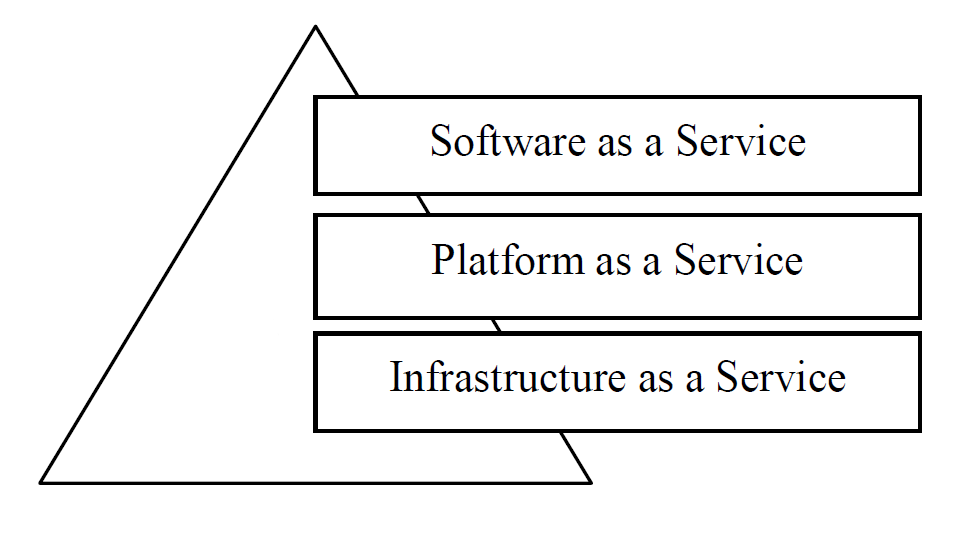
\includegraphics[width=0.7\linewidth]{images/cloud_computing_pyramide}
		\caption{3-Ebenen Modell von Cloud Computing}
		\label{fig:CloudComputingPyramide}
	\end{figure}


\textbf{Software as a Service (SaaS)} stellt eine Anwendung in der Cloud bereit, die von Nutzern verwendet werden kann, ohne eine eigene Installation vornehmen zu müssen. Der Nutzer hat dabei keinen Zugriff auf die Cloud Infrastruktur. Wichtige Merkmale einer SaaS Anwendungen sind Netzwerk basierter Zugriff, Nutzer können limitierte spezifische Konfigurationen vornehmen und sind meistens als Multi-Tenancy-System aufgebaut. Beispiele sind Anwendungen wie SalesForce.com, Google Mail, Google Docs, Office 365, Quicken Online, etc.
\\

\textbf{Platform as a Service (PaaS)} bezeichnet Software und Entwicklungs Tools die der Nutzer verwenden kann, um eigene Anwendungen zu entwickeln und zu veröffentlichen. Der Nutzer hat dabei keinen Zugriff auf die darunter liegende Cloud Infrastruktur, kann jedoch im Vergleich zu SaaS die eigene Anwendung frei konfigurieren. Beispiele für PaaS Services ist Google AppEngine.
\\

\textbf{Infrastructure as a Service (IaaS)} ist die unterste Ebene der Cloud Computing Pyramide. Dem Nutzer wird virtualisiert Hardware wie Datenspeicher, Virtuelle Maschinen, Netzwerke, etc. zur Verfügung gestellt, die frei verwendet werden können. IaaS Services werden gewöhnlich auf pay-per-use Basis bezahlt. Amazon EC2, VMWare und Windows Azure sind nur einige Beispiele.
\\

In einigen Fällen werden diese drei Ebenen noch um zusätzliche Service Formen ergänzt. So verwendet \cite[S. 28]{Tharam.2010} noch die Einteilung in storage as a Service (DaaS) während \cite[S. 123]{Mahmood.2011} von "other Provision as Service" spricht und darunter Formen wie Storage as a Service, Database as a Service, Security as a Service, Communication as a Service, etc gruppiert. All diese Services können jedoch auch spezialisierte IaaS Services angesehen werden.


\section{Bereitstellung Modell}
Ein weiterer zentraler Punkt in der Definition von Cloud Computing ist das Bereitstellungsmodell, das primär die Art beschreibt, wer Zugriff auf die Daten und Anwendungen hat.

	\begin{figure}[h]
		\centering
		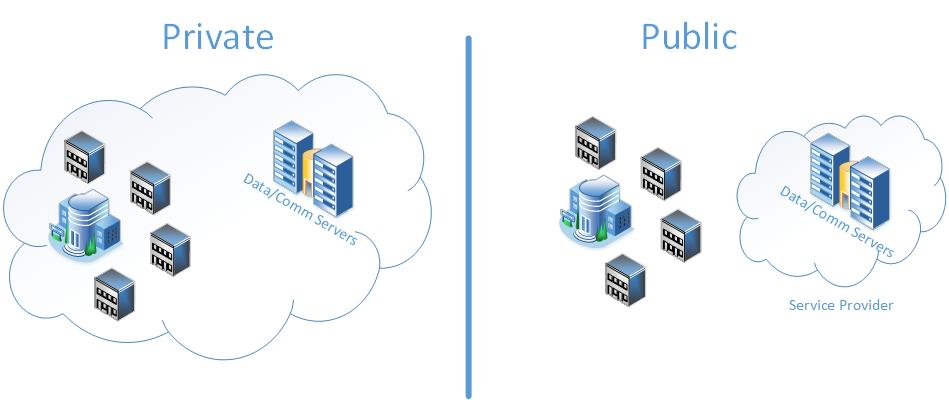
\includegraphics[width=0.9\linewidth]{images/private_public_cloud}
		\caption{Public und Private Cloud Architektur}
		\label{fig:PublicPrivateCloud}
	\end{figure}

\subsection{Private Cloud}
Als Private Cloud wird das Szenario beschrieben, wenn die Infrastruktur nur von einem Kunden genutzt wird. Im Normalfall ist sie im Organisationseigenen Rechenzentrum beheimatet. Sicherheit, Datenschutz, Wartung sind so einfacher durch eigenes Personal oder externe Dienstleister zu organisieren. Die Private Cloud lässt sich daher mit einem Intranet vergleichen. \cite[S. 879]{Jadeja.2012} \\
\cite{Tharam.2010} nennen fünf Gründe, die für eine Private Cloud sprechen können:
\begin{enumerate}
\item Maximieren und optimieren bestehender, eigenen Ressourcen
\item Sicherheitsbedenken und Datenschutz
\item Datentransferraten
\item Vollständige Kontrolle über kritische Aktivitäten
\item Forschungs- und Ausbildungszwecke
\end{enumerate}

\subsection{Public Cloud}
Dieses Modell ist derzeit am häufigsten verbreitet. Nutzer können die Cloud über ein Interface ansteuern und bezahlen für die Dauer der genutzten Services. Im Vergleich zu anderen Modellen ist die Public Cloud weniger sicher, da sie offen für bösartige Angriffe ist. Bekannte Public Cloud Anbieter sind Amazon EC2, S3, Google AppEngine, Force.com und Microsoft Azure. \\
(vgl. \cite{Jadeja.2012} und \cite{Tharam.2010})
	
\subsection{Hybrid Cloud}
Bei der Hybrid Cloud handelt es sich aus einer Kombination aus zwei oder mehr Cloud Arten, die für sich selbst existieren, aber miteinander verbunden sind. Dadurch lassen sich einfach eine Private und Public Cloud kombinieren, sodass Sicherheitsanforderungen gerecht geworden werden kann ein "outsourcing" weniger kritischer Teile in eine Public Cloud jedoch nichts im Wege steht.\\
Hybrid Clouds sind die Treiber zur Notwendigkeit einer Standardisierung und Cloud Interoperabilität.

	\begin{figure}[h]
		\centering
		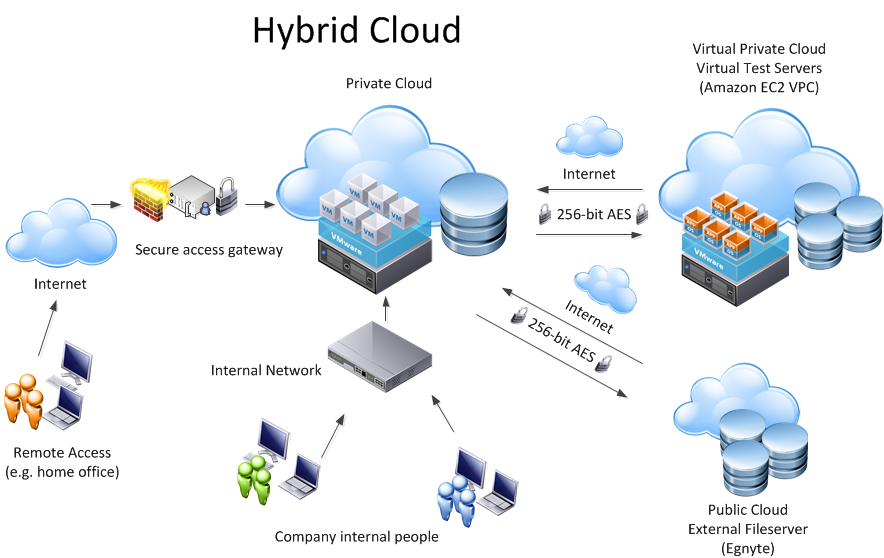
\includegraphics[width=0.9\linewidth]{images/hybrid-cloud-architektur}
		\caption{Hybrid Cloud Architektur}
		\label{fig:HybridCloud}
	\end{figure}


Community Cloud\\

\section{Pro \& Contra}
Nachdem der Begriff Cloud Computing, sowie die beinhalteten Service und Bereitstellungs Modelle erläutert wurden stellt sich die Frage nach den Vor- und Nachteilen dieses neuen Modelles. Wie bei den meisten neuen Technologien und Entwicklungen ist die Entstehung getrieben aus den Unzulänglichkeiten bestehender Ansätze und so können die Merkmale, die diese Neuentwicklung definieren in den meisten Fällen auch als Vorteile angesehen werden. Nachdem einige Gründe der Notwendigkeit bereits in Abschnitt~\ref{herausforderungen} erläutert wurden sollen hier die Vor- und Nachteile jedoch noch einmal explizit zusammen gefasst werden. Der Fokus liegt hierbei vor allem auf den Services IaaS und PaaS, die etwas anders betrachtet werden können als SaaS. Auch wenn viele der Vor- und Nachteile auch für SaaS Modelle gelten, werden diese im Abschnitt~\ref{SaaS} noch einmal explizit betratet. Verglichen werden dabei Cloud Anbieter mit dem traditionellen Rechenzentrum.

\subsection{Vorteile}

\subsubsection{Einfachheit}\label{einfachheit}
Cloud Angebote leben von ihrer einfachen Einrichtung. Speziell als Anwender bzw. Kunde genügt in den meisten Fällen ein Webbrowser, um sich auf der entsprechenden Oberfläche die benötigten Ressourcen anzufordern und automatisiert bereit gestellt zu bekommen. Es handelt sich hier um eine Art Outsourcing, sodass die Fachkenntnis auf Hardware- und Softwareebene nicht mehr in der Tiefe notwendig ist, wie sie bei einem eigenen Betrieb vorhanden sein muss, um ein gleichen Qualitätslevel zu erreichen.
\subsubsection{Kostenersparnis}\label{kostenersparnis}
Der Faktor Kostenersparnis ist wohl einer der größten Vorteile, wobei die Berechnung der Kostenersparnisse für IT nicht all zu trivial, da sich je nach Modell diese ggf. erst nach Jahren rentieren. Die Kosten im eigener Verantwortung gegeben sich primär aus den Beschaffungskosten für Hardware und Software und zusätzlich anteilig an den Personal- oder Dienstleister Kosten für Wartung und Instandhaltung. Mit einbezogen werden muss dabei jedoch auch, dass ggf. Neuanschaffungen und Erweiterungen über die Jahre notwendig sind.\\
 Die Preismodelle von Cloud Anbietern wie Amazon Web Services (AWS), Microsoft Azure (Azure) oder Google AppEngine (AppEngine) unterscheiden sich dabei sehr von den Traditionellen Abrechnungsmodellen. Auch wenn nicht jeder Anbieter alle Modelle unterstützt, so haben sich sich doch Abrechnungen nach Datenvolumen (wie viel Speicherplatz wird bereit gestellt), Computer Ressourcen (wie viel Arbeitsspeicher und CPU wird beansprucht), Datentransfervolumen (wie viel Datenvolumen wird über das Netzwerk transferiert) und einige Andere in der Praxis etabliert. Der große Unterschied liegt jedoch im Zusammenhang mit der Skalierbarkeit. So wird im Gegensatz zum traditionellen Rechenzentrum nur das bezahlt, was wirklich benutzt wird und überschüssige Ressourcen können bei bedarf einfach zurück gegeben werden. In der Literatur gibt es für diese Abrechnungsform jedoch bisher keinen Einheitlichen Begriff und wird als utility-style pricing, pay-as-you-go oder pay-per-use bezeichnet. (vgl. \citeauthor*[S. 879]{Jadeja.2012}; \citeauthor*[S. 313]{Achimugu.2012}) \\
 Wie groß die Kostenersparnisse im Detail sein können ist sehr abhängig von den Preisen, der Anwendungsarchitektur und der kalkulierten Laufzeit. In den letzten Jahren hat sich bei den Anbietern Amazon, Microsoft und Google ein richtiger Preiskrieg entwickelt, der zu stetig fallenden Preisen geführt hat und so die Kostenersparnisse weiter vergrößert hat. 

\subsubsection{Skalierbarkeit und Flexibilität}\label{skalierbarkeit}
Elastizität und Skalierbarkeit ist ein weiter Hauptvorteil von Cloud Umgebungen. Datenspeicher und Computing Power steht in fast unbegrenzter Menge zur Verfügung und kann mit wenigen Handgriffen vom User über einen Self-Service dazu provisioniert werden. So wie die Erweiterung der Ressourcen einfach möglich ist, so lassen sich diese auch wieder zurück geben wenn sie nicht mehr benötigt werden. Zusammen mit einer pay-per-use Abrechnung führt dies dazu, dass zusätzlich Ressourcen ggf. nur für bestimmte Zeiträume in Anspruch genommen werden müssen. \\
In traditionellen Rechenzentren ist dies schwieriger. Werden neue Ressourcen benötigt, so stehen diese nur begrenzt zur Verfügung. Durch unterschiedliche Virtualisierung Umgebungen hat dies zwar auch zu mehr Flexibilität geführt, jedoch sind die Möglichkeiten begrenzt. Auch die Zeit, die bis zur Bereitstellung neuer Ressourcen benötigt wird ist im Normalfall deutlich länger, da der Prozess weniger automatisiert abläuft.

\subsubsection{Zukunfts- und Ausfallsicherheit}\label{zukunftssicherheit}
Ausfälle von Hardware ist in der IT ein Fakt der sich nicht vermeiden lässt und unterscheidet sich nicht in Cloud und eigenen Rechenzentren. Gerade in den großen Rechenzentren mit tausenden von Servern ist die Wahrscheinlichkeit für ein auftreten eines solchen Ausfalles natürlich deutlich höher. Mit Redundanz und das Vermeiden von single point of failures wird in Rechenzentren versucht den Hardware Ausfall für den Endkunden unsichtbar zu machen und den Betrieb ungestört aufrecht erhalten zu können. \\
Durch die reine Anzahl von Hardware und spezialisiertem Personal sind die Cloud Anbieter in ihren Rechenzentren hier deutlich im Vorteil einen störungsfreien Betrieb zu garantieren. Zudem ist durch den Austausch kaputter oder veralteter Hardware eine sukzessive Erneuerung der Hardware ohne weiter Kosten für den Endkunden gegeben.

\subsubsection{Nachhaltigkeit}\label{nachhaltigkeit}
Green IT, der umweltschonende Betrieb und Herstellung von Informationstechnologie, ist in den letzten Jahren von immer größerer Bedeutung geworden. Cloud Computing kann in diesem Bereich einiges beitragen, da Energiekonzepte einfacher optimiert und Ressourcen besser genutzt werden können. \citeauthor*{Siegele.2008} geht von einer durchschnittlichen Auslastung von Hardware Ressourcen mit 5\%-20\% in traditionellen Rechenzentren aus. Was auf den ersten Blick sehr wenig erscheint begründet sich darin, das in Lastspitzen die benötigten Ressourcen um ein 2 bis 10-faches steigen. Um diesen Anforderungen gerecht zu werden, wird in vielen Fällen eine Provisionierung auf Basis des maximalen Workloads vorgenommen und führt zur Ressourcenverschwendung in weniger aktiven Zeiten.\\
Durch das einfache hinzufügen von Ressourcen und die interne Ressourcen Verwaltung modernen Cloud Rechenzentren kann dies die Auslastung der einzelnen Systeme auch bei geringer oder moderater Belastung verbessern und so seinerseits zur Umweltschonung beitragen. 

\subsubsection{Beispiel}
Diese Vorteile lassen sich an einem kleinen Beispiel im Hochschulsport mit fiktiven Zahlen verdeutlichen. Wie bereits in Abschnitt~\ref{hspAnforderungen} beschrieben kommt es zu einem enormen zusätzlichen Performance Bedarf für das Buchungssystem zum Buchungsstart. Als Lastspitze wird ein Bedarf von 100 Servern zu Grunde gelegt. Diese Lastspitzen treten etwa 10 mal im Jahr auf und halten für 24 Stunden an. Den Rest der Zeit besteht ein Workload für etwa 20 Server. Daraus ergibt sich über das Jahr ein durchschnittlicher Bedarf an Serverstunden von 532,6 je Tag. Für eine Veranschaulichung des Kostenfaktors wird eine Serverstunde mit 50 Cent veranschlagt.
\\
\\
Serverstunden je Tag => ((355 * 20) + (10 * 100)) * 24 / 365 = 532,6 \\
Kosten je Tag => (532,6 * 50) / 100 = 266,3€ \\

Um den Kunden auch in den Lastspitzen die benötigte Performance zusichern zu können, so müsste in einer traditionellem Rechenzentrum die Bemessung des Bedarfs am Peak Load erfolgen und somit für 100 Server. Gemessen am durchschnittlichen Bedarf über das Jahr stellt dies jedoch eine deutliche Überprovisionierung da. (BILD)
	\begin{figure}[h]
		\centering
		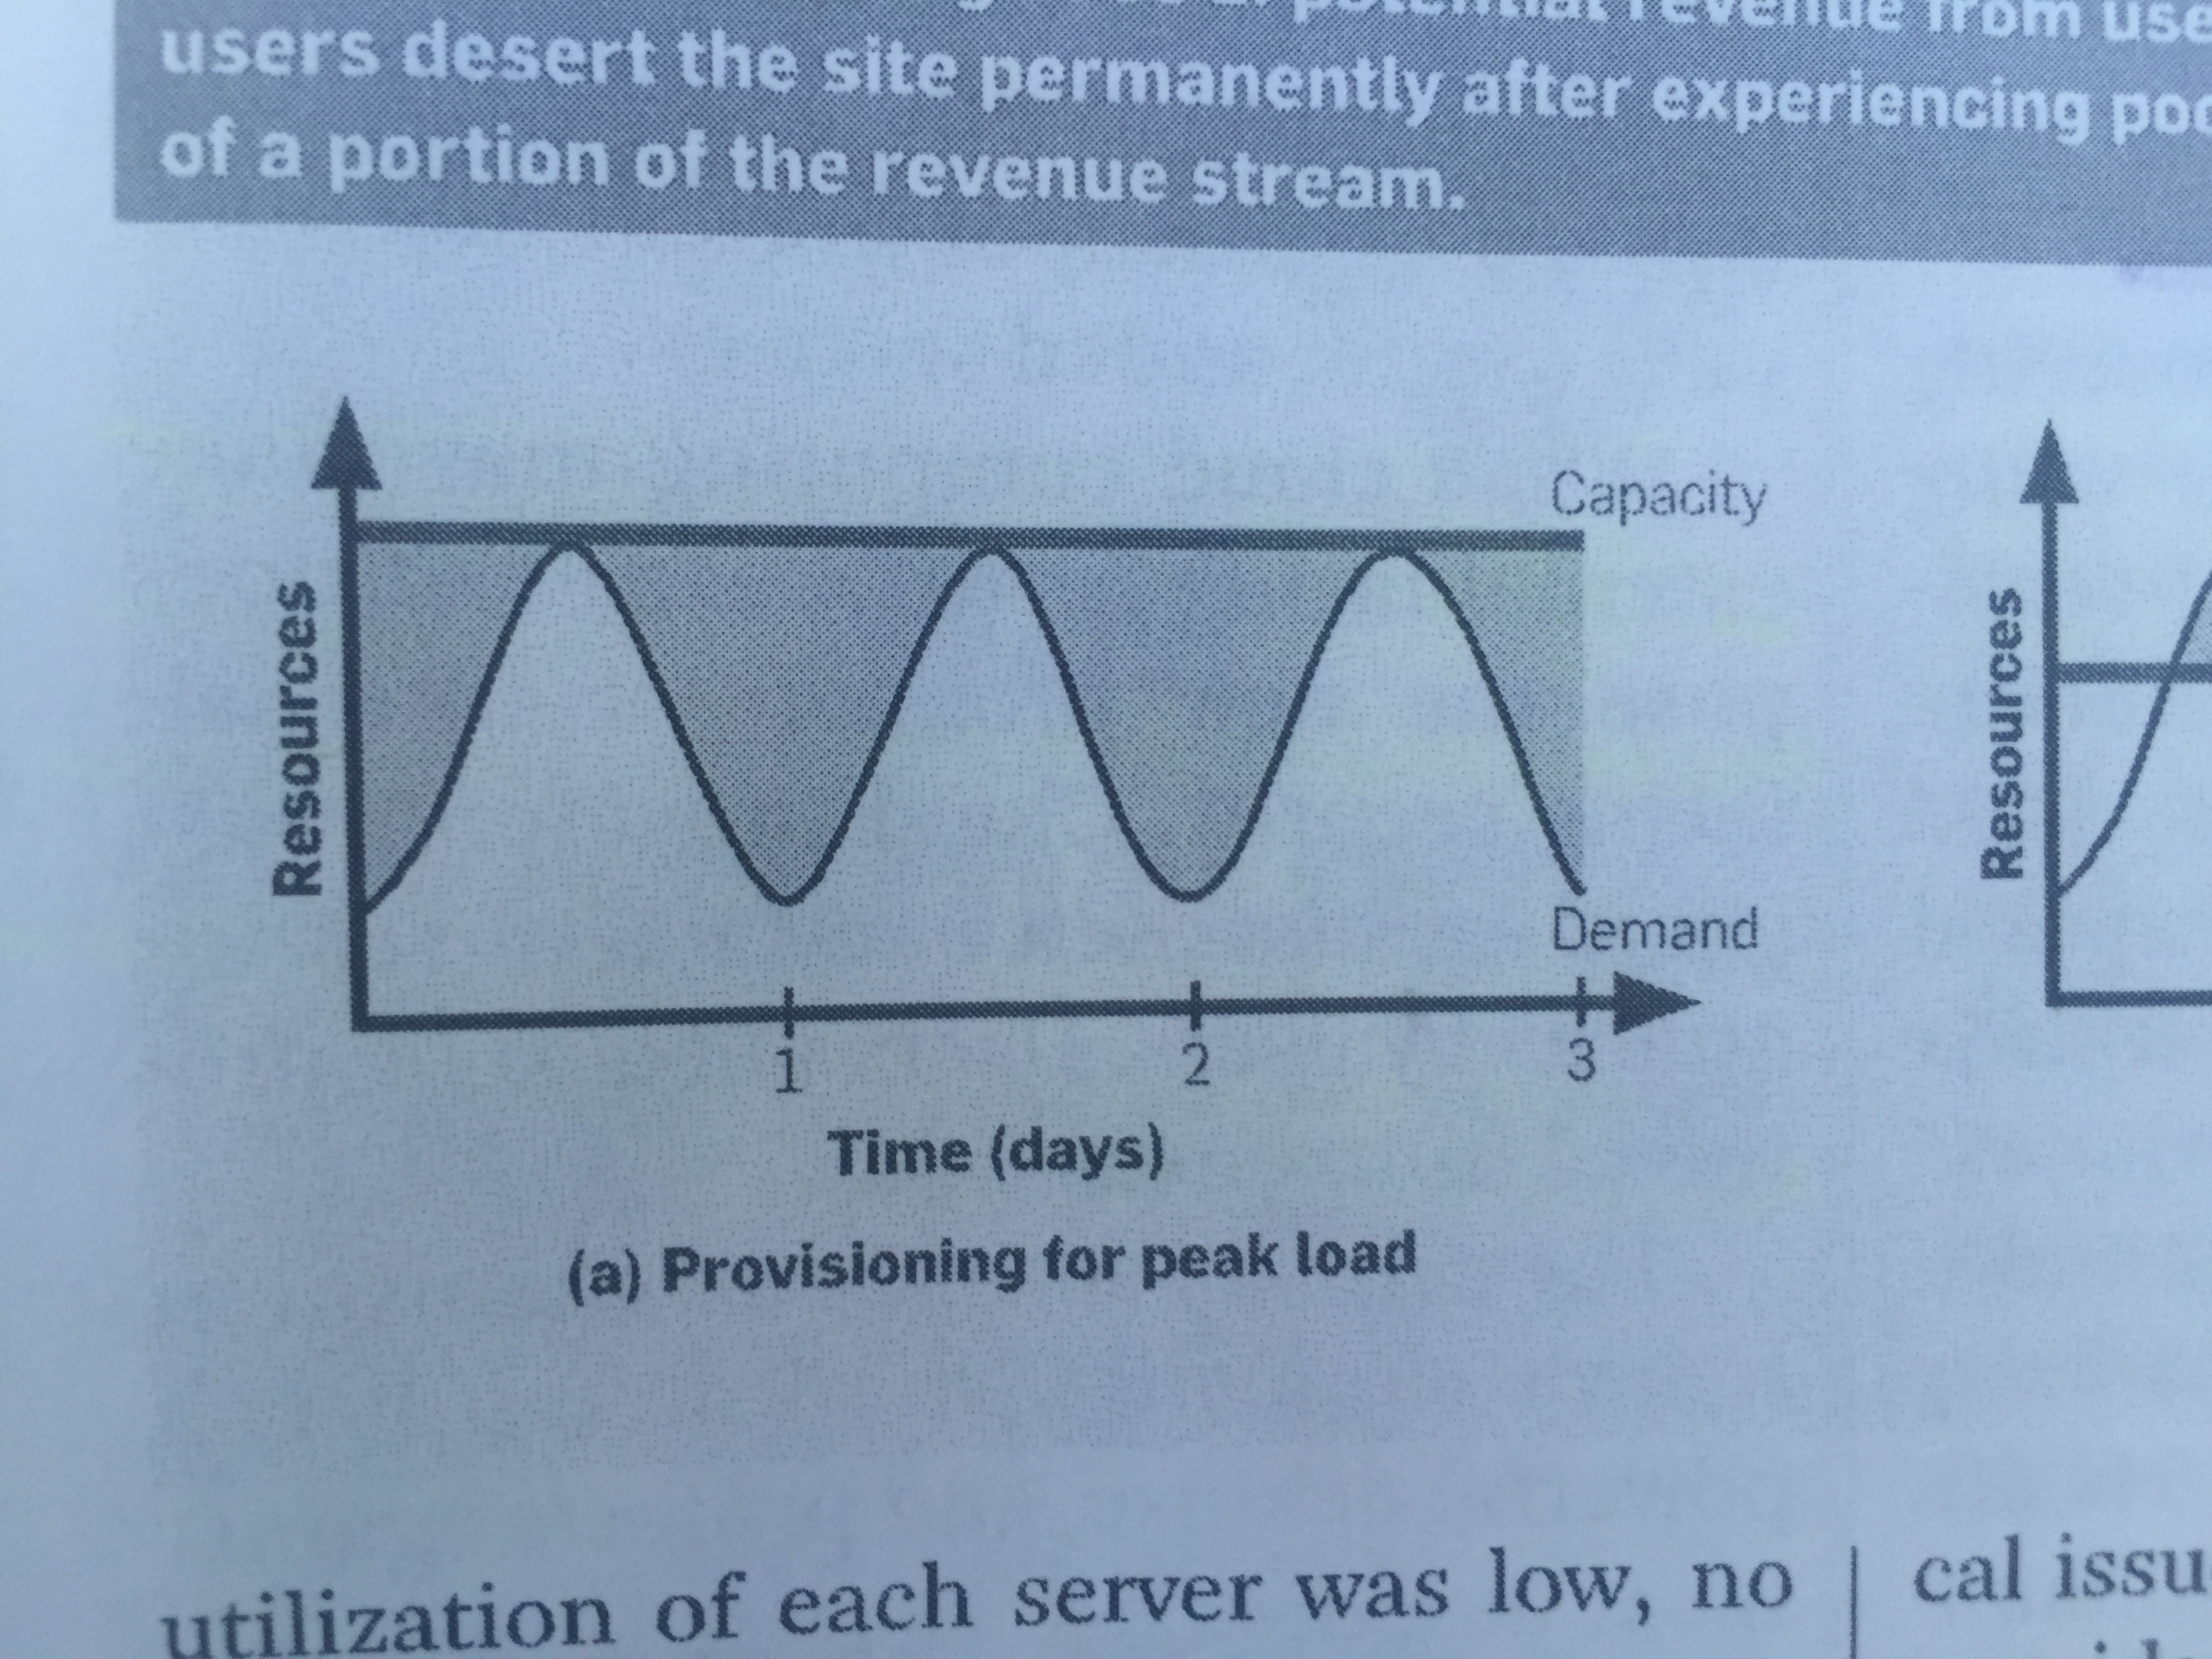
\includegraphics[width=0.7\linewidth]{images/overprovisioning}
		\caption{Provisionierung für Lastspitzen}
		\label{fig:overprovisioning}
	\end{figure}
\\ 
\\
Serverstunde je Tag => 100 * 24 = 2400 \\
Kosten je Tag => (2400 * 50) / 100 = 1200€ \\ 
\\
Dies Entspräche einer Faktor von 4,5.
\\
Ein alternativer Ansatz wäre eine moderatere Bemessung des Bedarfes möglich mit z.B. 50 Servern und somit einer Unterprovisionierung. Dies würde dazu führen, das die Lastspitzen jedoch nicht mehr entsprechend versorgt werden könnten und es zu Einschränkungen und sogar Ausfällen des System kommen könnte. 
	\begin{figure}[h]
		\centering
		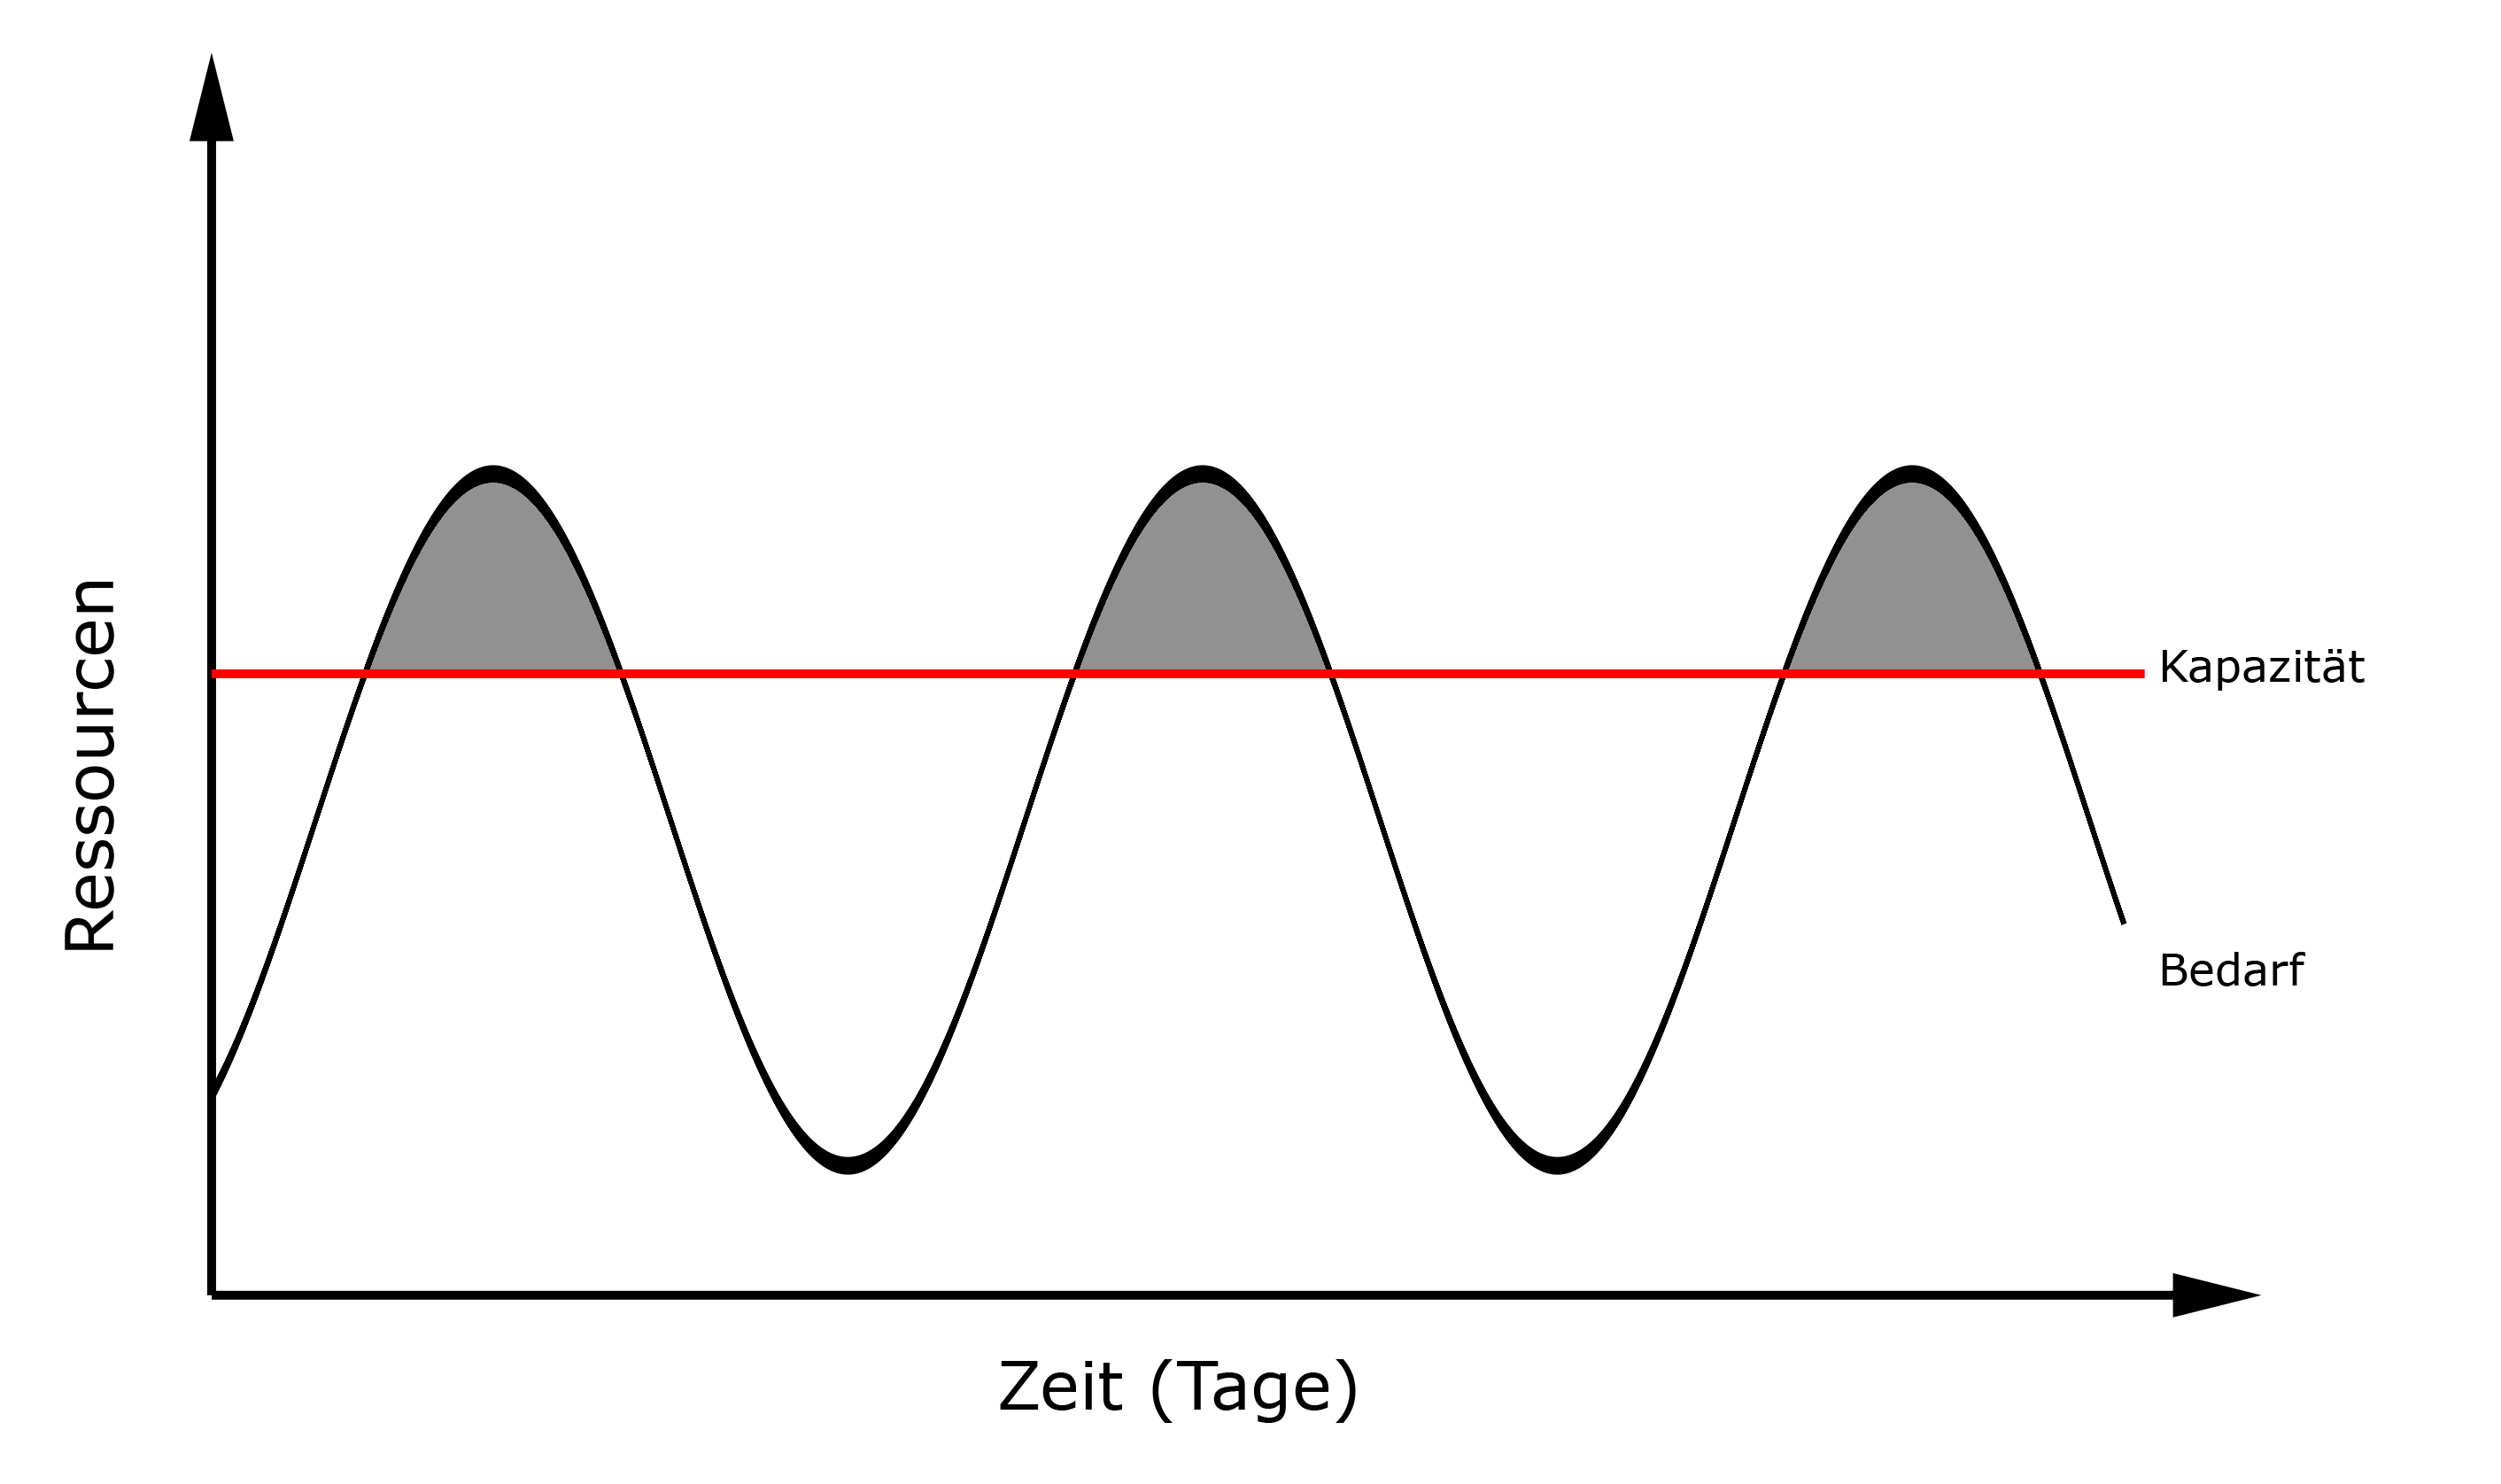
\includegraphics[width=0.7\linewidth]{images/underprovisioning}
		\caption{Unterprovisionierung}
		\label{fig:underprovisioning}
	\end{figure}
Mit diesem Ansatz ließen sich deutliche Einsparungen erzielen, jedoch muss mit betrachtet werden, dass es zu deutlichen Einnahme Einbußen kommen könnte, da nicht allen Kunden eine Buchung möglich wäre oder sich Kunden sogar vollständig vom diesem Dienst entfernen.
\\
\\
Serverstunde je Tag => 50 * 24 = 1200 \\
Kosten je Tag => (1200 * 50) / 100 = 600€ \\
\\ 

Dieses auf fiktiven Zahlen basierende Beispiel ist in der realen Welt häufig anzutreffen und es müssen mit dem traditionellen Modell Kompromisse eingegangen werden, die unterschiedlich stark ausfallen können. Kosten-Nutzen-Optimierungen sind immer notwendig, bekommen mit dem Cloud Computing aber neue Möglichkeiten. Eine Umsetzung im Cloud Umfeld könnte wie folgt aussehen. Um einen reibungslosen Betrieb in den Phasen mit weniger Aktivität zu gewährleisten und einen gewissen Puffer zu integrieren, werden für das Jahr 25 Server provisioniert. Für die Anmelde Zeiträume werden jeweils für 48 Stunden weiter 75 Server dazu geschaltet. Daraus ergäbe sich folgende Rechnung:
\\
\\
Serverstunden je Tag => ((355 * 25) + (20 * 100)) * 24 / 365 = 715,07 \\
Kosten je Tag => (715,07 * 50) / 100 = 357,53€ \\

Dies entspräche dem 1,34-fachem des durchschnittlichen Bedarfes und ist in erster Linie dem Puffer geschuldet. Im Vergleich zur Überprovisionierung betragen die Kosten aber nur das 0,3-fache und im Vergleich zur Unterprovisionierung das 0,6-fache ohne die einhergehenden Geschäftlichen Verluste.
Dieses vereinfachte Beispiel macht so klar, welche Vorteile vor allem die Punkte Kosteneinsparung, Skalierbarkeit und Flexibilität in Cloud Umgebungen bringen.

\subsection{Nachteile}
Neben den bereits genannten Vorteilen haben sich neue Technologien und Modelle meist mit einigen Problemen und Herausforderungen auseinander zu setzen, die hier ebenfalls vorgestellt werden sollen.
\subsubsection{Sicherheit und Datenschutz}

\subsubsection{Abhängigkeit}

\subsubsection{Internetzugang}
Da alle Cloud Dienste über das Internet angebunden werden, ergibt sich eine zusätzliche Internet Abhängigkeit, die ein Arbeiten bei gestörten Verbindungen unmöglich macht. Ob die Störung dabei beim Kunden oder beim Anbieter liegt ist dabei unerheblich. Im Vergleich zu den traditionellen eigenen Rechenzentren erhöht sich damit die Komplexität und die Anforderungen an die Internet-Bandbreite, die in lokalen Netzwerken leichter bereit gestellt werden konnte.
\subsubsection{Verfügbarkeit}
Die Zuverlässigkeit eines Anbieters gilt weiter als Nachteil, da mehr Schnittpunkte existieren. Ausfälle bei Amazon, Microsoft oder Google können zum Ausfall aller Systeme führen. Es muss dabei aber gesagt werden, das diese Ausfälle auch in lokalen Rechenzentren jederzeit passieren und passieren können. Die Ausfallzeiten der etablierten Anbieter beschränkte sich in den letzten Jahren auf ein Minimum (QUELLE?)

\subsubsection{Interoperabilität}
Viele Cloud-Anbieter bieten je nach Service viele eigenen Techniken, Produkte und Services mit denen gearbeitet wird. Prinzipiell ist dabei ein Umzug zu einem anderen Cloud Anbieter nicht vorgesehen, da es zu Inkompatibilitäten führen kann. Dies kann zu großen Problemen führen, wenn diese Anbieter ggf. insolvent gehen oder der Kunde aus anderen Gründen den Anbieter wechseln möchte. 

\section{SaaS Anwendungen}
\subsection{Monolitische versus service basierte Architekturen}
\subsection{Herausforderungen}
\subsubsection{Availability}
\subsubsection{Data management}
\subsubsection{Design and Implementation}
\subsubsection{Messaging}
\subsubsection{Management and Monitoring}
\subsubsection{Performance and Scalability}
\subsubsection{Resiliency}
\subsubsection{Security}


